%% LyX 2.0.2 created this file.  For more info, see http://www.lyx.org/.
%% Do not edit unless you really know what you are doing.
\documentclass[12pt,twoside,english]{report}
\usepackage{lmodern}
\renewcommand{\familydefault}{\rmdefault}
\usepackage[T1]{fontenc}
\usepackage[latin9]{inputenc}
\usepackage[a4paper]{geometry}
\geometry{verbose,tmargin=3.5cm,bmargin=3cm,lmargin=3.5cm,rmargin=3cm,footskip=1cm}
\usepackage{fancyhdr}
\pagestyle{fancy}
\setcounter{secnumdepth}{3}
\setcounter{tocdepth}{3}
\setlength{\parskip}{\medskipamount}
\setlength{\parindent}{0pt}
\usepackage{float}
\usepackage{textcomp}
\usepackage{amsmath}
\usepackage{graphicx}
\usepackage{setspace}
\usepackage[authoryear]{natbib}
\usepackage{nomencl}
% the following is useful when we have the old nomencl.sty package
\providecommand{\printnomenclature}{\printglossary}
\providecommand{\makenomenclature}{\makeglossary}
\makenomenclature
\usepackage{subscript}
\setstretch{1.5}

\makeatletter

%%%%%%%%%%%%%%%%%%%%%%%%%%%%%% LyX specific LaTeX commands.
%% Because html converters don't know tabularnewline
\providecommand{\tabularnewline}{\\}
%% A simple dot to overcome graphicx limitations
\newcommand{\lyxdot}{.}


%%%%%%%%%%%%%%%%%%%%%%%%%%%%%% User specified LaTeX commands.
\usepackage{fancyhdr}
\pagestyle{fancy}
\fancyhead[RE]{\bfseries \nouppercase\leftmark}
\fancyhead[LO]{\bfseries \nouppercase \rightmark}

\renewcommand{\chaptermark}[1]{%
\markboth{\chaptername 
\ \thechapter\ }{}}

 
\fancyhead[LE,RO]{\bfseries\thepage}
\fancyfoot{}
\raggedbottom
\setlength{\parindent}{8mm}

\makeatother

\usepackage{babel}
\begin{document}

\chapter{A SOM of the Australian Region\label{chap:Regional-SOM}}

\newpage{}


\section*{Summary}

\noindent This chapter examines the common synoptic weather regimes
of the Australian region by means of a Self-Organising Map (SOM) of
the Mean Sea-Level Pressure (MSLP) field from the European Centre
for Medium-range Weather Forecasts (ECMWF) product, ERA-Interim. An
examination of the SOM technique's effectiveness is undertaken, along
with the presentation of an improvement to the use of the SOM in this
thesis.

\noindent \newpage{}


\section{Introduction\label{sec:SOM-Regnl-Intro}}

This chapter presents the results from training SOMs of various sizes
and initial values with MSLP data from ERA-Interim, and for the whole
domain covering Australia with dimensions (6�S,105�E) \textrightarrow{}
(49.5�S,165�E). The SOM of the whole domain is shown to be consistent
with other studies using the technique for the Austral region. However,
in the current study there is no expectation that offshore locations
be utilised for wind or solar power as the vast majority of the Australian
coastline has steep ocean floor gradients (\citealp{Diesendorf2006}).
Hence an alternative SOM that utilises only the data over the Australian
continent is also presented. The alternative SOM is also shown to
be more effective at classifying the original data. This chapter is
structured as follows. Section \ref{sec:Creating-the-SOM} describes
the results (both whole and continental domains), section \ref{sub:Alternative-SOMs}
presents an alternative SOM formulation, mapping of the SOM back onto
the data is described in \ref{sub:Mapping-the-SOM} and following
the filtering of the mapping the tendencies of the SOM created are
explored in \ref{sub:Analysis-of-Regional}. Finally, a discussion
and summary are given in section \ref{sec:SOM-Conclusion}.


\section{Creating the SOM \label{sec:Creating-the-SOM}}

The whole domain SOM (land and ocean grid points) was created by simply
showing all of the available MSLP data to the training process. However,
the continental SOM was created by only analysing the variability
over the Australian continent. The domain for the continental version
was also reduced to exclude some of the land north of the Australian
continent that was included in the whole domain version. The refined
domain, (10.5�S, 105�E) \textrightarrow{} (49.5�S, 165�E), for the
continental version is shown in Fig. \ref{fig:Map-Continent}.
\begin{figure}[H]
\begin{centering}
\includegraphics{\string"/home/rhuva/Robert/Final Thesis/Chapter 5/Figures/LSM_comp_HIRES_continents_contour\string".eps}
\par\end{centering}

\caption{Map of the extended land-sea mask used for filtering the ERA-Interim
ocean variability. Areas coloured orange are included in the analysis
of continental Australia. \label{fig:Map-Continent}}
\end{figure}


The mask used for filtering out the ocean variability was an altered
version of the land-sea mask variable supplied by ECMWF. When compared
to the Interactive Data Language \nomenclature{IDL}{Interactive Data Language}(IDL)
map of the Australian continent, the ECMWF-supplied land-sea mask
variable appeared not to include some areas of the Australian continent
as land. The decision was then made to extended the ECMWF land-sea
mask variable to include all grid-boxes that appeared to contain land
in the IDL map, which was of finer detail.

Table. \ref{tab:SOM-training-list} describes the final whole domain
results and Table. \ref{tab:SOM-Init-Params} the continental domain
results following the two phases of training described earlier. The
term \textquotedblleft{}averaged quantised error\textquotedblright{}
refers to the Euclidean distance (sum of squared differences---the
equivalent of Eq. \ref{eq:ERA-RMSE-BMU} multiplied by $\sqrt{n}$)
between each time step in the data and its respective Best Matching
SOM node (BMU), averaged over all time steps. Throughout the thesis
the quantised error measurement is used to compare time steps with
their closest matching SOM node. The pattern correlation technique
was tested for this purpose, however was not seen to perform any better
than quantised error/Euclidean distance measure (not shown). The main
weakness of the pattern correlation technique was its insensitivity
to magnitude. The SOM dimensions listed in Tables. \ref{tab:SOM-training-list}
and \ref{tab:SOM-Init-Params} are some of the possible combinations
that follow the advice from the software---that the extent of one
spatial dimension always be bigger than the other (\citealp{Kohonen1995}).
Indeed there are any number of possible SOM shapes (for instance,
\citet{Alexander2010} used a SOM with four columns and five rows).
The shape of the SOM (number of rows and columns) is predetermined
by the user. 
\begin{table}[h]
\begin{centering}
\begin{tabular}{|c|c|c|c|}
\hline 
SOM dimensions & Initial alpha & Initial radius & Average quantised error (hPa)\tabularnewline
\hline 
\hline 
3 nodes (3x1) & 0.15 & 1 & 212.0\tabularnewline
\hline 
8 nodes (4x2) & 0.2 & 2 & 189.6\tabularnewline
\hline 
15 nodes (5x3) & 0.3 & 3 & 169.9\tabularnewline
\hline 
20 nodes (5x4) & 0.8 & 4 & 165.4\tabularnewline
\hline 
24 nodes (6x4) & 0.5 & 4 & 161.9\tabularnewline
\hline 
30 nodes (6x5) & 0.7 & 5 & 157.1\tabularnewline
\hline 
35 nodes (7x5) & 1.0 & 5 & 154.1\tabularnewline
\hline 
42 nodes (7x6) & 0.6 & 6 & 150.7\tabularnewline
\hline 
48 nodes (8x6) & 0.04 & 6 & 148.9\tabularnewline
\hline 
\end{tabular}
\par\end{centering}

\caption{List of initial radius and initial alpha combinations for each SOM
size that produced the smallest average quantised error. \label{tab:SOM-training-list}}
\end{table}
\begin{table}[H]
\begin{centering}
\begin{tabular}{|c|c|c|c|}
\hline 
SOM dimensions & Initial alpha & Initial radius & Average quantised error (hPa)\tabularnewline
\hline 
\hline 
3 nodes (3x1) & 0.2 & 1 & 88.0\tabularnewline
\hline 
8 nodes (4x2) & 0.55 & 2 & 74.5\tabularnewline
\hline 
15 nodes (5x3) & 1.0 & 3 & 66.0\tabularnewline
\hline 
20 nodes (5x4) & 1.0 & 4 & 62.4\tabularnewline
\hline 
24 nodes (6x4) & 1.0 & 4 & 60.9\tabularnewline
\hline 
30 nodes (6x5) & 0.5 & 5 & 58.8\tabularnewline
\hline 
35 nodes (7x5) & 0.3 & 5 & 57.6\tabularnewline
\hline 
42 nodes (7x6) & 0.4 & 6 & 56.1\tabularnewline
\hline 
48 nodes (8x6) & 0.1 & 6 & 55.3\tabularnewline
\hline 
\end{tabular}
\par\end{centering}

\caption{As per Table. \ref{tab:SOM-training-list}, except using the continental
data.\label{tab:SOM-Init-Params} }
\end{table}


Twenty random initialisations for each whole domain SOM in training
phase one were also experimented with to test for convergence of the
final results. The random initialisation, however, was seen to have
very little effect on the final average quantised error for each radius-alpha
combination (all differences were in the range of \textpm{}2.94hPa
for the whole domain). It is thought that even though various random
initialisations were explored, the final run length (306,800) is long
enough to produce approximately the same SOM space in spite of any
differences in initialisation. 

After forming the list of \textquoteleft{}best\textquoteright{} SOMs
in Tables. \ref{tab:SOM-training-list} and \ref{tab:SOM-Init-Params}
a process for deciding which SOM size to use for later calculations
was undertaken. The aim of the decision process for SOM size was to
determine which of the above SOM sizes represented enough of the data
space to accurately describe MSLP variability over the Austral domain,
but at the same time did not have too many nodes to easily visualise.
\citet{Hewitson2002} in their proposal for the use of SOMs in climatology
suggested that a subjective choice can be just as effective as a mathematical
criterion for selecting the \textquoteleft{}optimum\textquoteright{}
number of nodes to use. This suggestion by \citet{Hewitson2002} was
brought about by the observation that the same broad groupings appear
with all SOM sizes and that the number of nodes simply determines
the degree of generalisation---a characteristic that was also observed
in the current study (not shown).

Despite this assertion from \citet{Hewitson2002}, there are known
and tested methods for objectively or even semi-objectively determining
how many sub-groupings of a data set is the optimal amount (see \citealp{Tibshirani2001}
for examples). For instance, conventional clustering analysis provides
many proposed methods for determine how many clusters to utilise.
But given that the SOM technique does not cluster in the traditional
sense and instead represents a smooth continuum of nodes that span
the data-space, such techniques from clustering analysis were not
seen to be entirely applicable to the SOM technique, and thus not
applicable to this thesis.

As noted by \citet{Sugar1998} the \textquoteleft{}elbow\textquoteright{}
phenomenon is a common way of determining the point at which the addition
of more clusters/nodes gives no appreciable increase in the amount
of the data-space represented by all clusters/nodes. In terms of the
analysis presented in the current study, such an \textquoteleft{}elbow\textquoteright{}
could be determined by graphing the number of nodes versus the average
quantised error for each SOM size (Fig. \ref{fig:Decay-of-average}).
\begin{figure}[H]
\begin{centering}
\includegraphics{\string"Figures/Decay of error\string".eps}
\par\end{centering}

\caption{Decay of average quantised error (blue) and the progression of the
change-in-gradient (red) versus the number of nodes used for a) the
whole domain and b) the continental domain. The change-in-gradient
was calculated by the centred difference method. \label{fig:Decay-of-average}}
\end{figure}


As can be seen from Fig. \ref{fig:Decay-of-average}a, there does
appear to be a small but noticeable \textquoteleft{}elbow\textquoteright{}
in the whole domain graph at point (15, 169.9), which is also seen
in the change-in-gradient maximum. However, and despite the \textquoteleft{}elbow\textquoteright{}
from Fig. \ref{fig:Decay-of-average}a, other studies from the Australian
region (for instance \citealp{Alexander2010}; \citealp{Hope2006};
\citealp{Verdon-Kidd2009}) suggest more than 15 nodes are required
to appropriately describe the synoptic influences over Australia.
Thus a finding by the elbow method that 15 nodes were \textquoteleft{}enough\textquoteright{}
to properly represent the data was questionable. 

From initial inspection it was found that a SOM with 48 nodes was
much too cumbersome to visualise, while a SOM with three nodes was
clearly not representative of the variation in synoptic patterns over
the last 21 years. To determine which of the SOM sizes from the intermediate
range of possible sizes to employ, an index was proposed. The current
study asserts that an index that takes into account the number of
nodes used as well as the average quantised error of each SOM size
can easily be formulated and implemented by Eq. \ref{eq:Number-of-nodes}. 

\begin{equation}
n=max\left\{ \frac{(qerror_{max}-qerror_{n})\cdot(n_{max}-n)^{2}}{(qerror_{n}-qerror_{min})\cdot qerror_{n}}\right\} \label{eq:Number-of-nodes}
\end{equation}


where $n$ is the number of nodes, $n_{max}$the maximum number of
nodes trialled,$qerror$ represents the average quantised error, $qerror_{max}$
the maximum $qerror$ value, $qerror_{min}$ the minimum $qerror$
value and $qerror_{n}$ the $qerror$ value for each $n$.

Eq. \ref{eq:Number-of-nodes} is a balance between the numerator,
which rewards fewer nodes, and the denominator, which rewards smaller
quantised errors. Using the values from Tables. \ref{tab:SOM-training-list}
and \ref{tab:SOM-Init-Params} reduces Eq. \ref{eq:Number-of-nodes}
to: 

\begin{equation}
n=max\left\{ \frac{\mid212hPa-qerror_{n}\mid\cdot\,(48-n)^{2}}{(qerror_{n}-148.9hPa)\cdot qerror_{n}}\right\} =30\,\, nodes,\,\, and\label{eq:Eq4-solution}
\end{equation}


\noindent 
\begin{equation}
n=max\left\{ \frac{(88hPa-qerror_{n})\cdot(48-n)^{2}}{(qerror_{n}-55.3hPa)\cdot qerror_{n}}\right\} =30\,\, nodes\label{eq:Number-Nodes-SOM-Cont}
\end{equation}


Both Eqs. \ref{eq:Eq4-solution} and \ref{eq:Number-Nodes-SOM-Cont}
explain that a SOM with 30 nodes has the \textquoteleft{}optimum\textquoteright{}
balance between the competing factors of SOM size and SOM error for
their respective domains. When graphed, the maximum at 30 nodes for
Eqs. \ref{eq:Eq4-solution} and \ref{eq:Number-Nodes-SOM-Cont} is
clearly visible (Figs. \ref{fig:Graph-of-Equation}a and \ref{fig:Graph-of-Equation}b).
\begin{figure}[H]
\begin{centering}
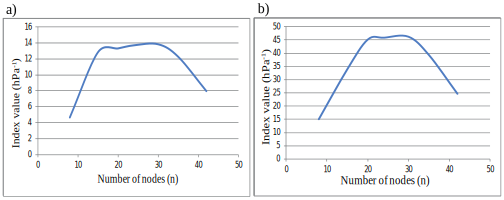
\includegraphics{Figures/number_nodes}
\par\end{centering}

\caption{a) Graph of Eq. \ref{eq:Eq4-solution} using the values from Table.
\ref{tab:SOM-training-list} and b) graph of Eq. \ref{eq:Number-Nodes-SOM-Cont}
using values from Table. \ref{tab:SOM-Init-Params}.\label{fig:Graph-of-Equation}}
\end{figure}


Using the results from Eqs. \ref{eq:Eq4-solution} and \ref{eq:Number-Nodes-SOM-Cont},
the SOMs with 30 nodes and parameters described in Tables. \ref{tab:SOM-training-list}
and \ref{tab:SOM-Init-Params} were chosen to represent the 21 year
period 1989-2009 of ERA-Interim MSLP variability for the whole domain
Austral region (Fig. \ref{fig:6x5-SOM-space}) and continental region
(Fig. \ref{fig:6x5-SOM-space-Cont}). 
\begin{figure}[h]
\begin{centering}
\includegraphics{Figures/SOM_MSLP_all_6x5_alpha0\lyxdot 7_bubble_large}
\par\end{centering}

\caption{6x5 SOM space for the Austral region using ERA-Interim MSLP data from
1989-2009 and with boundaries described earlier. Horizontal axes are
in units of degrees longitude and vertical axes are in units of degrees
latitude. \label{fig:6x5-SOM-space}}
\end{figure}
\begin{figure}[h]
\begin{centering}
\includegraphics{\string"/home/rhuva/Robert/Final Thesis/Chapter 5/Figures/SOM_MSLP_cont_6x5_alpha0.5_bubble_large\string".eps}
\par\end{centering}

\caption{6x5 SOM space of the 1989-2009 ERA-Interim MSLP over the Australian
continent. \label{fig:6x5-SOM-space-Cont}}
\end{figure}


As can be seen from Fig. \ref{fig:6x5-SOM-space} there is a clearly
defined continuum of synoptic classifications that range from low-pressure
intrusions on the left hand side to high pressure intrusions on the
right hand side. The features of the whole domain SOM from Fig. \ref{fig:6x5-SOM-space}
are in accordance with other studies using the SOM technique with
MSLP; for instance, \citet{Hewitson2002}, \citet{Alexander2010}
and \citet{Hope2006}. Transitional phases between episodes of high
and low pressure dominance are also visible in Fig. \ref{fig:6x5-SOM-space},
while the \textquoteleft{}traditional\textquoteright{} west-to-east
cycle between successive high pressure systems is possible if one
traces out the SOM perimeter in a clockwise fashion. The continental
SOM (Fig. \ref{fig:6x5-SOM-space-Cont}) also displays one corner
of the SOM space occupied by higher pressure, consistent with the
subtropical ridge, with the opposite corner dominated by lower pressure.
In the case of the continental SOM, the SOM nodes that represent the
low pressure systems to the south are not readily discernible. However,
it is still clear that the general characteristics of the Australian
region (like that seen in the whole domain version) are captured in
the continental version. In some sense the SOMs in the continental
version are cut-outs, in the shape of the Australian continent, of
the whole domain SOM.


\subsection{Alternative SOMs\label{sub:Alternative-SOMs}}

For regions that exhibit large seasonality in meteorological conditions
it might make more sense to conduct the training of the SOM with seasonally
partitioned data (consequently also one SOM for each season). For
the Australian region there are indeed some previous studies in which
the seasonal partitioning is undertaken (see \citet{Alexander2010}
and \citet{Huva2014}). In such studies the SOM is used to study characteristics
of the MSLP field, and related fields, solely from that season. Indeed
the southern regions of Australia exhibit seasonality in pressure
such that certain phenomena (see Fig. \ref{fig:Gallant-SE-Aus-Teleconnetions})
occur more commonly in winter as opposed to summer, and vice versa.
However, what was found in this thesis was little difference in the
resulting SOM when the data was partitioned into seasons. Fig. \ref{fig:JJA-6x4-SOM}
illustrates this relative insensitivity to season by using the same
domain and time period from the previous regional example (Fig. \ref{fig:6x5-SOM-space}),
except using only wintertime data.
\begin{figure}[H]
\noindent \centering{}\includegraphics{Figures/SOM_MSLP_JJA_6x4_alpha0\lyxdot 06_bubble-journal}\caption{A SOM of wintertime (June, July and August) MSLP for 1989-2009 ERA-Interim.
Optimum parameters were 24 nodes with initial alpha of 0.06.\label{fig:JJA-6x4-SOM}}
\end{figure}


The size and optimum parameter combination utilised in Fig. \ref{fig:JJA-6x4-SOM}
was determined using the same processes outlined in the previous section
(Section \ref{sec:Creating-the-SOM}). What is seen in Fig. \ref{fig:JJA-6x4-SOM}
are very similar features to the version of the SOM using all available
data. The features seen in Fig. \ref{fig:JJA-6x4-SOM} are also similar
to the previous studies of the Australian region using only wintertime
data (\citet{Huva2014}; \citet{Alexander2010}). Unfortunately though
the use of just the wintertime data has not made a drastic difference
to the level of low pressure intrusion into the domain. Instead the
wintertime SOM contains just the more northerly centred high pressure
systems, along with the transition states (ridging high pressure)
at latitude \textasciitilde{}35-40�S and cold fronts with a more upright
structure (nodes 12, 15-16 and 19-24). It is suggested that the time
period used (21 years) is sufficiently long enough to smoothen the
influence of even predominantly winter-only synoptic weather types
(for instance, cut-off lows). It is therefore a reasonable expectation
for the wintertime SOM to struggle capturing the fast moving and intense
low pressure systems that the annual SOM also has no closely resembling
node for (cut-off and east coast lows). 

The intention with this thesis is to study the year-round influential
synoptic weather types for RE production over Australia. The infrastructure
needed to capture the RE output analysed in this thesis would also
be subject to the full annual array of weather types and not available
to be moved with the seasons. In this instance splitting the SOM typing
into seasons would make less sense. It is also overwhelmingly more
common in the literature to conduct the training of the SOM for the
Australian region with all available data (\citet{Brown2010,Hope2006,Jiang2011,Nicholls2009,Verdon-Kidd2009}).Thus
the remainder of this thesis will focus on just the occurrence of
the annual SOM nodes seen in Fig. \ref{fig:6x5-SOM-space-Cont}.


\section{Mapping the SOM\label{sub:Mapping-the-SOM}}

With the SOMs created it was possible to go back through the original
data-set and look at the characteristics of the SOM nodes through
time and their implications for other atmospheric variables like wind
speed and solar irradiance. In order to map the SOM nodes back onto
the original data-set a program from the SOM\_PAK described in \citet{Kohonen1995}
was employed. The program called \textquotedblleft{}visual\textquotedblright{}
from the SOM\_PAK was used to analyse the time steps from original
data-set and to assign each time step with a matching SOM node (the
BMU). The SOM node with the smallest Euclidean distance was chosen
as the node that \textquoteleft{}matched\textquoteright{} each time
step and thus the data-set of 30,680 time steps was reduced to a time
series of just 30 SOM nodes, or synoptic classes. However, given the
smooth nature of the SOM and the SOM\textquoteright{}s ability to
span the data-space, there were no time steps in the ERA-Interim reanalysis
that had an exactly matching BMU. Thus it was necessary to implement
a method for determining whether each of the 30,680 BMUs were indeed
an accurate match. The process of checking the BMUs also ensured that
the purpose of the current study---to determine the synoptic influences
on wind and solar output---was not undermined by falsely assigning
SOM nodes to conditions from the original data-set. 

Given that the SOM nodes are artificial and there is no direct knowledge
of the state of the atmosphere corresponding to each node\textquoteright{}s
pressure distribution, any process for checking the matching of SOM
nodes back onto the original data-set needs to be a function of pressure
only. However, it was not immediately apparent as to what criteria
or criterion should be used as an investigation of this sort appears
not to have been undertaken before with SOMs. To give an indication
as to how well or poor the SOM nodes map onto the ERA-Interim reanalysis
Fig. \ref{fig:SOM-comp-worst-before} shows for the whole domain,
and Fig. \ref{fig:SOM-Comp-Cont-Worst-Best} for the continental domain,
the BMUs with the smallest and largest quantised errors alongside
their respective time steps. 
\begin{figure}[h]
\noindent \begin{centering}
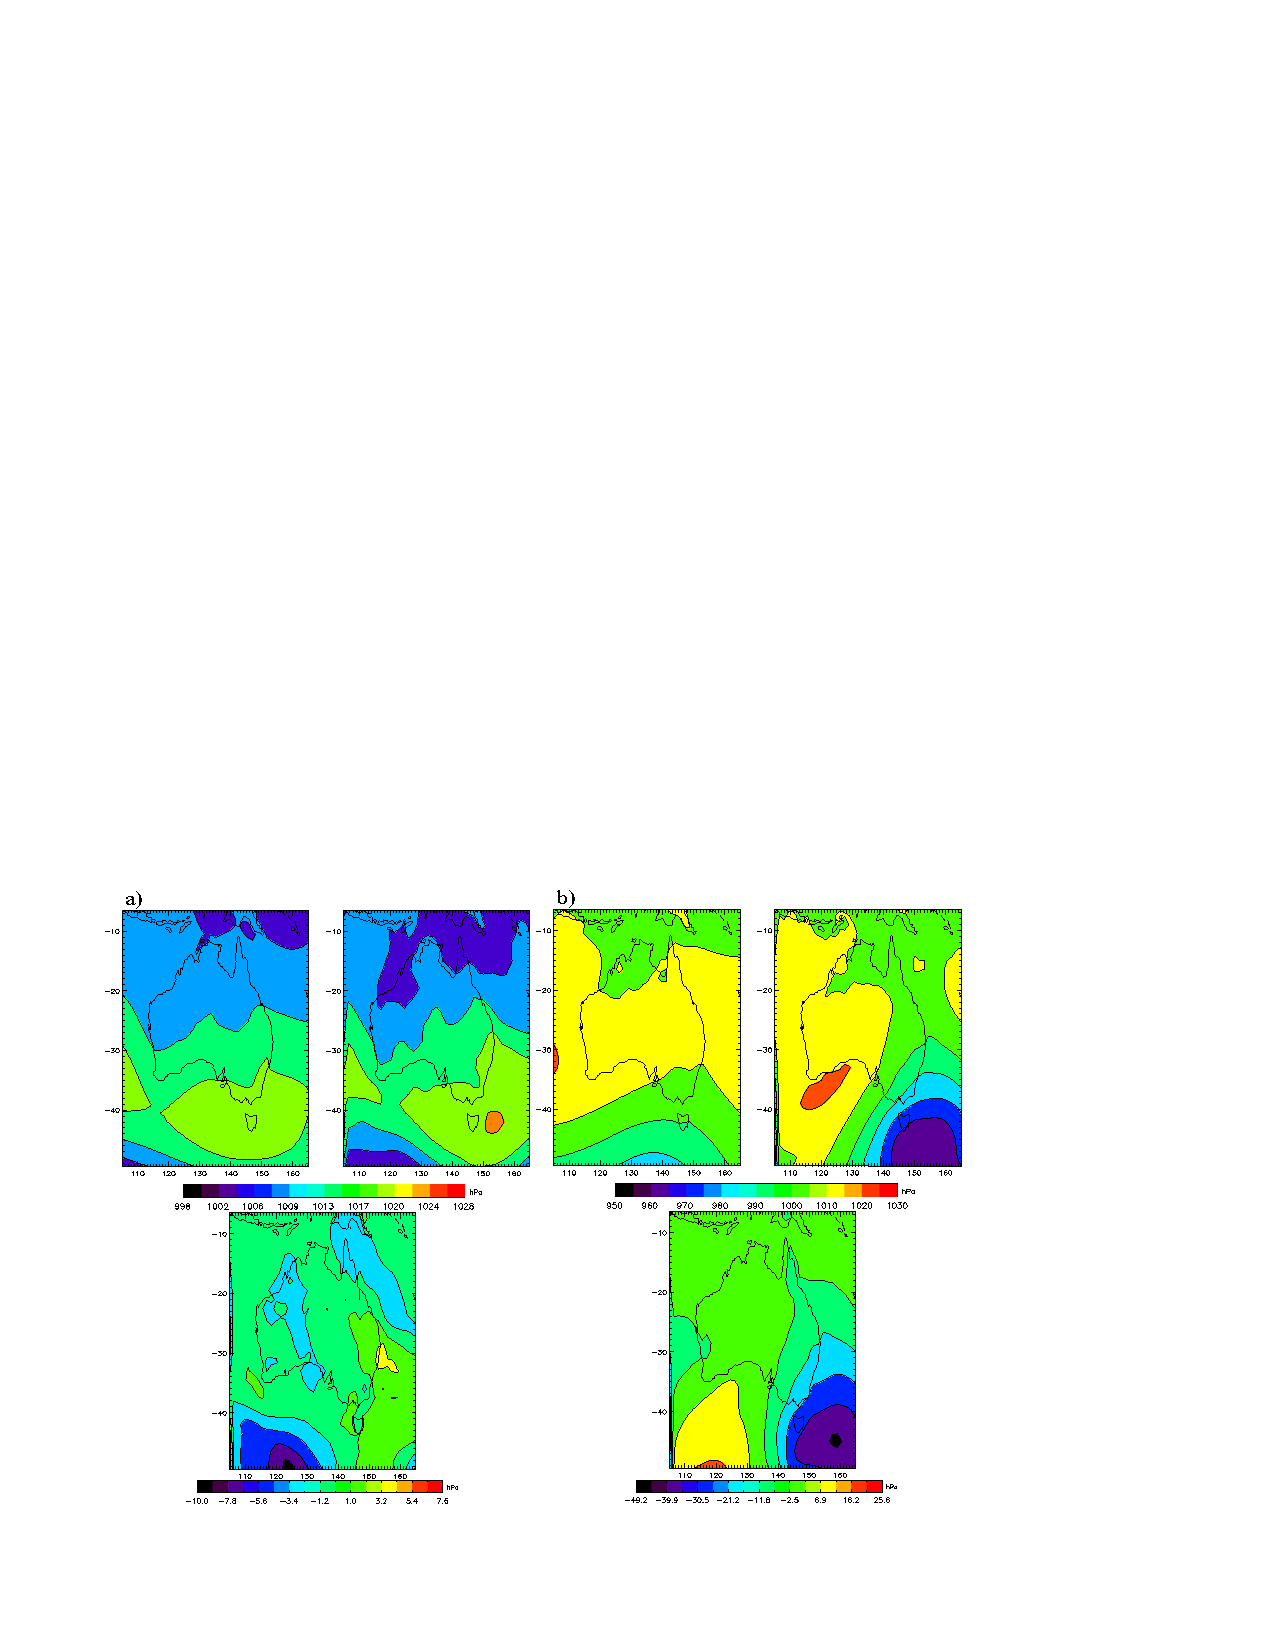
\includegraphics{Figures/SOM_comp_regnl_wrst_b4_filt}
\par\end{centering}

\caption{Comparison between the BMUs with the smallest a) and largest b) quantised
errors for the SOM from Fig. \ref{fig:6x5-SOM-space}. a) is a comparison
between node 10 and conditions at 1800UTC on March 11 2008 while b)
is a comparison between node 25 and conditions at 0600UTC on November
6 1994. The quantised error for a) is 59.2hPa, for b) is 428.6hPa
and the horizontal and vertical axes are in units of degrees longitude
and latitude, respectively. The bottom panel shows the difference
between the time step and its BMU (time step - BMU).\label{fig:SOM-comp-worst-before} }
\end{figure}
\begin{figure}[h]
\begin{centering}
\includegraphics{\string"/home/rhuva/Robert/Final Thesis/Chapter 5/Figures/SOM_cont_wrst_bst_b4_filt\string".eps}
\par\end{centering}

\caption{Comparison between the BMUs with the smallest a) and largest b) quantised
errors for the SOM from Fig. \ref{fig:6x5-SOM-space-Cont}. a) is
a comparison between node 13 and conditions at 1200UTC on April 15
1994 while b) is a comparison between node 24 and conditions at 0600UTC
on September 29 1996. The quantised error for a) is 16.6hPa, for b)
is 216.4hPa and the horizontal and vertical axes are in units of degrees
longitude and latitude, respectively. The bottom panel shows the difference
between the time step and its BMU (time step - BMU). \label{fig:SOM-Comp-Cont-Worst-Best}}
\end{figure}


As can be seen from both Fig. \ref{fig:SOM-comp-worst-before} and
\ref{fig:SOM-Comp-Cont-Worst-Best} the \textquoteleft{}best\textquoteright{}
BMUs match the pressure distribution of their respective time steps
very well. However, the `worst\textquoteright{} BMU for the whole
domain (Fig. \ref{fig:SOM-comp-worst-before}b) represents quite a
different pressure distribution, particularly in south-eastern Australia,
when compared to its respective time step. It is then intuitive to
suggest that counting the BMU from Fig. \ref{fig:SOM-comp-worst-before}b
as a \textquoteleft{}match\textquoteright{} would most likely be misrepresenting
the weather conditions on 0600UTC June 11 1994. From a visual inspection,
node 25 of the whole domain SOM is characterised by a high pressure
system that ridges across the Australian continent and therefore is
not expected to yield the windy and potentially cloudy conditions
for south-eastern Australia suggested by the MSLP map from 0600UTC
on June 11 1994. 

Fig. \ref{fig:SOM-Comp-Cont-Worst-Best} shows that the continental
SOM did a better job at matching just the variability over the continental
Australia. The BMU with the highest quantised error (Fig. \ref{fig:SOM-Comp-Cont-Worst-Best}b),
while still miss-matching the pressure distribution over south-eastern
Australia had a quantitative advantage by not including variability
over the ocean. This advantage was expected given the more southerly
nature of intense low pressure systems (those lows that do not represent
enough of data to have a SOM node that matches them closely). However,
as can be seen from Fig. \ref{fig:SOM-Comp-Cont-Worst-Best}b, there
were still instances where low pressures systems that did not look
like any of the SOM nodes from Fig. \ref{fig:6x5-SOM-space-Cont}
intrude on the Australian continent. The extent to which the discrepancy
in node-matching represented by Fig. \ref{fig:SOM-comp-worst-before}b
and Fig. \ref{fig:SOM-Comp-Cont-Worst-Best}b repeated throughout
the data-set was not a trivial question to answer.


\subsection{Filtering the Mapping\label{sub:Filtering-the-Mapping}}

It is, of course, possible to set an upper limit on the quantised
error or even other measures like the spatial correlation---thus disregarding
those matches that exceed the upper limit. But without the direct
knowledge of the state of the atmosphere suggested by each SOM node,
the cut-off point for considering whether or not the pressure distribution
from a BMU is not accurate enough is potentially fraught with subjectivity
(comparing each time step with its best matching SOM node). Thus an
investigation was undertaken to understand the disparity between \textquoteleft{}good\textquoteright{}
and \textquoteleft{}poor\textquoteright{} matches through time and,
in particular, to reveal whether it was possible to define a relatively
easy set of criteria that ensured \textquoteleft{}poor\textquoteright{}
matches were discarded. 

To give an indication as to how the BMU quantised error values are
partitioned throughout the data, Figs. \ref{fig:SOM-ordered-histo}
and \ref{fig:SOM-Cont-Ordered-Histo} show both the graph of ordered
values and the histogram of quantised errors for the whole domain
(Fig. \ref{fig:SOM-ordered-histo}) and continental SOMs (Fig. \ref{fig:SOM-Cont-Ordered-Histo}).
\begin{figure}[h]
\begin{centering}
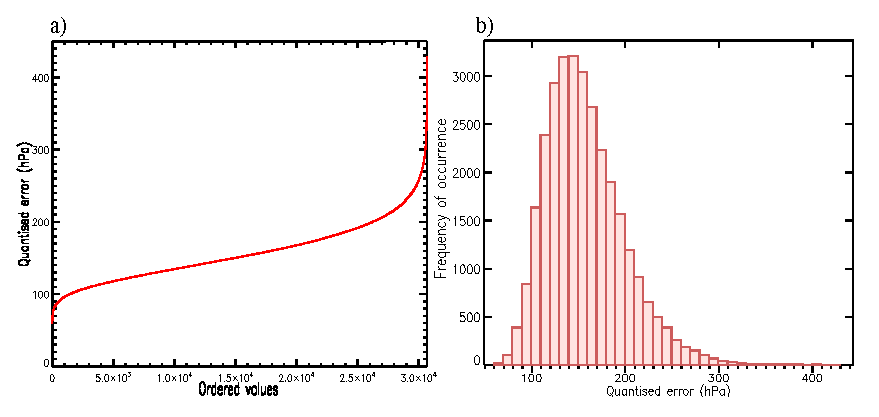
\includegraphics{Figures/SOM_regnl_ordered_histo}
\par\end{centering}

\caption{Graph of a) ordered BMU quantised errors and b) histogram of BMU quantised
errors for the SOM shown in Fig. \ref{fig:6x5-SOM-space}. \label{fig:SOM-ordered-histo}}
\end{figure}
\begin{figure}[h]
\noindent \begin{centering}
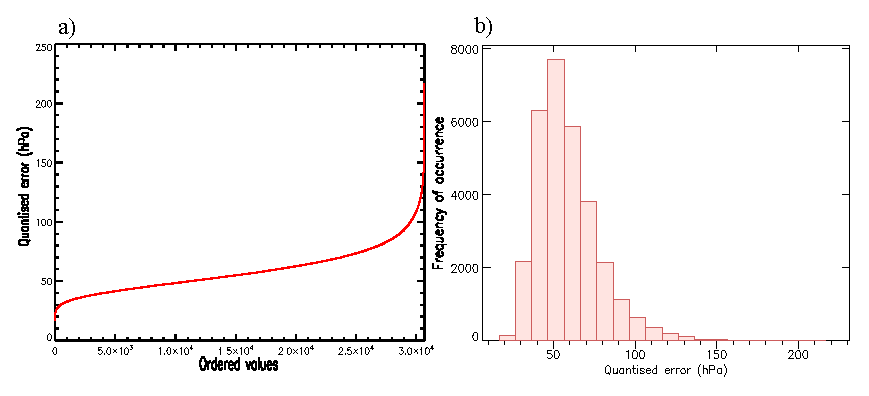
\includegraphics{Figures/SOM_cont_ordered_histo}
\par\end{centering}

\caption{As per Fig. \ref{fig:SOM-ordered-histo}, except for the continental
BMUs.\label{fig:SOM-Cont-Ordered-Histo}}
\end{figure}


As Figs. \ref{fig:SOM-ordered-histo} and \ref{fig:SOM-Cont-Ordered-Histo}
reveal, the distribution of quantised error is quite positively skewed
and has only a small portion of BMUs with error greater than about
200hPa for the whole domain and 100hPa for the continental domain
(less than half the respective maxima in quantised error). Thus Figs.
\ref{fig:SOM-ordered-histo} and \ref{fig:SOM-Cont-Ordered-Histo}
suggest that most of the \textquoteleft{}poor\textquoteright{} matches
could be removed by eliminating only a small percentage of the total
BMU matches. 

As a starting point, Figure 17a from \citet{Dee2011} shows that the
maximum Root Mean Square Error \nomenclature{RMSE}{Root Mean Square Error}(RMSE)
of southern hemisphere surface pressure in the ERA-Interim reanalysis
is approximately 1.75hPa in the early 1990\textquoteright{}s (not
shown). Assuming a similar error in MSLP (which is derived using the
surface pressure, average virtual temperature and constants) and considering
the equation for RMSE in pressure, it was possible to equate the RMSE
using observations (Eq. \ref{eq:ERA-RMSE-obs}) with the RMSE using
the BMUs (Eq. \ref{eq:ERA-RMSE-BMU})---the resulting value could
then be thought of as a minimum threshold for keeping BMUs. Noting
the existence of the Euclidean distance term in the numerator of Eq.
\ref{eq:ERA-RMSE-BMU} and using the value of 1.75hPA for RMSE\textsubscript{obs},
it was argued that any BMU with a Euclidean distance (quantised error)
less than 61.4hPa was within the error of the ERA-Interim reanalysis
and thus should be kept. The quantised error value of 61.4hPa was
thus a minimum criterion to be used. However, only three of the BMUs
for the Austral domain had a quantised error below 61.4hPa and thus
nearly all BMUs were outside the error of the ERA-Interim reanalysis.
\begin{equation}
RMSE_{obs}=\frac{\sqrt{\overset{n}{\underset{i=0}{\sum}}(P_{ERA,\, i}-P_{obs,\, i})^{2}}}{\sqrt{n}}=1.75hPa\label{eq:ERA-RMSE-obs}
\end{equation}


where $n$ is the number of observations used to calculate the error,
$P_{obs}$ represents the pressure value from the $n^{th}$ observation
and $P_{ERA}$ represents the pressure value in ERA-interim at the
nearest grid-point to the location of the observation.
\begin{equation}
\begin{array}{ccc}
RMSE_{BMU} & = & \frac{\sqrt{\overset{n}{\underset{i=0}{\sum}}(P_{ERA,\, i}-P_{BMU,\, i})^{2}}}{\sqrt{n}}\end{array}\label{eq:ERA-RMSE-BMU}
\end{equation}


where $n$ is now the number of grid-points in the ERA-Interim Austral
domain and $P_{BMU}$ represents the pressure value from the $n^{th}$
grid-point in each BMU. The conversion from ERA-Interim error to BMU
quantised error is thus:

\noindent \begin{center}
$\begin{array}{cccc}
if\,\,\,\,1.75hPa & = & \frac{\sqrt{\overset{n}{\underset{i=0}{\sum}}(P_{ERA,\, i}-P_{BMU,\, i})^{2}}}{\sqrt{n}}\\
\\
1.75hPa\cdot\sqrt{n} & = & \sqrt{\overset{n}{\underset{i=0}{\sum}}(P_{ERA,\, i}-P_{BMU,\, i})^{2}}\,\,\,\,\,= & Quantised\,\,\, error\\
then\,\,\,1.75hPa\cdot\sqrt{1230} & = & Quantised\,\,\, error\,=\,\,61.4hPa
\end{array}$
\par\end{center}

With nearly all BMUs having a quantised error larger than the error
of the ERA-Interim reanalysis, an analysis of the maximum discrepancy
(largest single grid-point error) across the domain for each BMU and
its respective time-step was conducted in order to help determine
how many BMUs to discount as \textquoteleft{}matches\textquoteright{}.
The analysis of the maximum discrepancy (single grid-point errors)
for all whole domain BMUs revealed a mean maximum discrepancy of 16.9hPa---the
smallest maximum discrepancy was 5hPa and the largest maximum discrepancy
was 52.1hPa. As per the distribution in Fig. \ref{fig:SOM-ordered-histo}b,
the histogram of maximum discrepancies for the whole domain was also
quite positively skewed with the mode at 9hPa but the mean and median
at 16.9hPa and 16.1hPa, respectively (not shown). It was then thought
that a relatively easy way to identify BMUs that had pressure distributions
too different from their matched time step was to eliminate the BMUs
with a maximum discrepancy greater than or equal to 20hPa; 20hPa was
chosen as the cut-off value because it represented a balance between
keeping as many matches as possible (to aid later statistical analyses)
and not keeping matches that had very obvious MSLP differences. Choosing
a cut-off criterion that was based on analysing single grid-point
errors also gave some insight into the spatial distribution of errors,
which is not possible using the quantised error measurement due to
the aggregation of error. This initial filtering of the BMUs left
22,962 matches out of a total 30,680 for the whole domain, and left
30,108 matches for the continental domain. The whole domain BMU with
the largest quantised error from the BMUs that remained after the
initial filtering is depicted in Fig. \ref{fig:SOM-Comp-Aft-Filt-1}
and for the continental domain is depicted in Fig. \ref{fig:SOM-Comp-Cont-Aftr-Filt1}.
\begin{figure}[h]
\begin{centering}
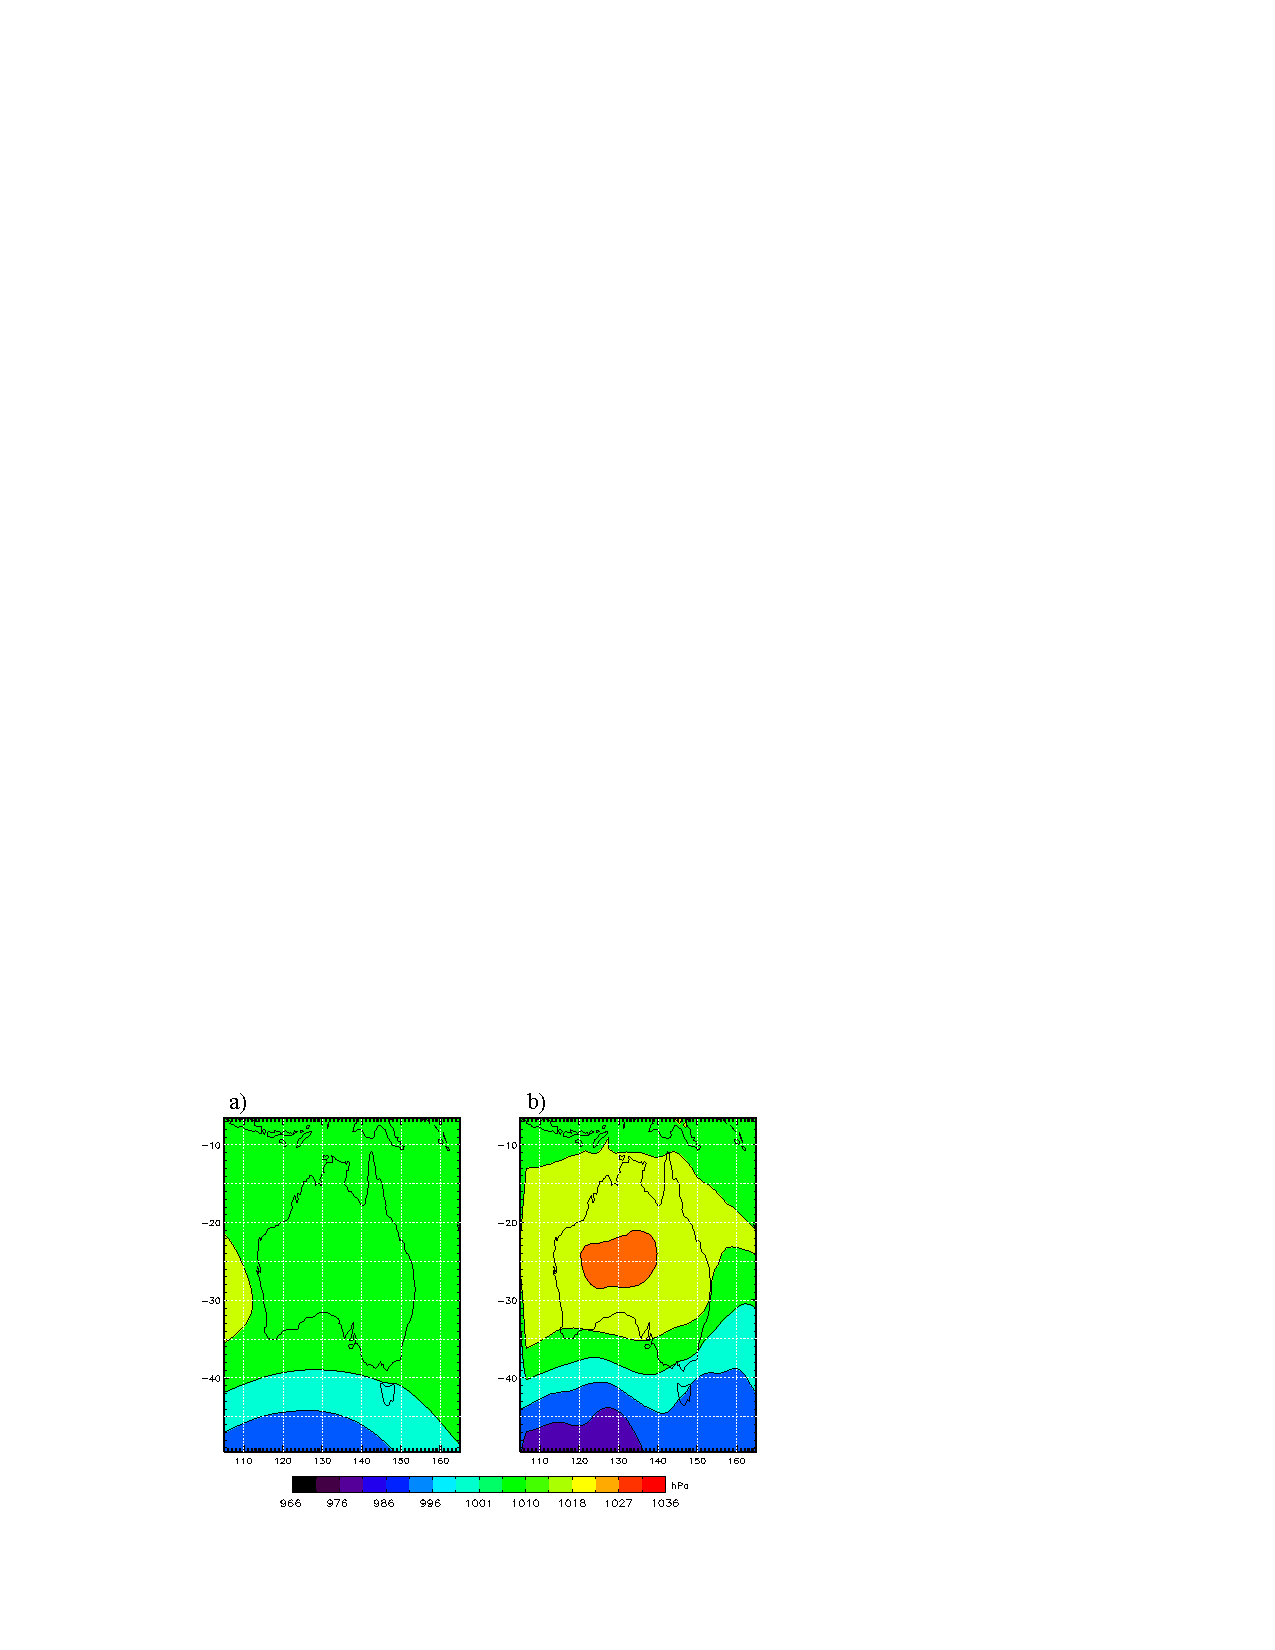
\includegraphics{Figures/SOM_comp_regnl_wrst_aft_filt_1}
\par\end{centering}

\caption{Comparison between a) node 19 from the SOM depicted in Fig. \ref{fig:6x5-SOM-space}
and b) the MSLP map from 0000UTC on July 4 2002. The quantised error
between a) and b) is 296.8hPa. The horizontal and vertical axes are
in units of degrees longitude and latitude, respectively.\label{fig:SOM-Comp-Aft-Filt-1}}
\end{figure}
\begin{figure}[H]
\begin{centering}
\includegraphics{\string"/home/rhuva/Robert/Final Thesis/Chapter 5/Figures/SOM_cont_wrst_aft_filt_I\string".eps}
\par\end{centering}

\caption{Comparison between a) node seven from the SOM depicted in Fig. \ref{fig:6x5-SOM-space-Cont}
and b) the MSLP map from 0000UTC on June 14 2000. The quantised error
between a) and b) is 158.4hPa. \label{fig:SOM-Comp-Cont-Aftr-Filt1}}
\end{figure}


As can be seen from Figs. \ref{fig:SOM-Comp-Aft-Filt-1} and \ref{fig:SOM-Comp-Cont-Aftr-Filt1},
the \textquoteleft{}worst\textquoteright{} BMU after the initial filtering
represent less obviously different pressure distributions than was
seen in Figs. \ref{fig:SOM-comp-worst-before}b and \ref{fig:SOM-Comp-Cont-Worst-Best}b.
However, a quick inspection of the BMUs with a similarly large quantised
error as those in Figs. \ref{fig:SOM-Comp-Aft-Filt-1} and \ref{fig:SOM-Comp-Cont-Aftr-Filt1}
revealed that indeed some of the other \textquoteleft{}poorer\textquoteright{}
matches still had pressure distributions indicative of largely different
weather conditions across much of the southern and south-eastern Australian
continent (not shown). Analysing the distribution of quantised errors
after filtering (Figs. \ref{fig:SOM-Ordered-histo-after-filt1}a and
\ref{fig:SOM-Ordered-histo-after-filt1}b) revealed much the same
behaviour seen in Figs. \ref{fig:SOM-ordered-histo} and \ref{fig:SOM-Cont-Ordered-Histo},
and thus the decision was made to eliminate BMUs with quantised errors
in the highest 5\% (the `worst' 5\%). The amount of BMUs left after
this second filtering was 21,814 for the whole domain and 28,602 for
the continental domain. Obvious, already, was the fact that the continental
domain was far out-performing the whole domain SOM in terms of the
number of matches that were surviving the filtering. The continental
domain SOM had many more BMU whose pressure distributions closely
matched their SOM node (mostly due to the limited domain that contained
less low pressure intrusions), thus also enhancing later statistical
analysis involving the occurrence of SOM nodes.
\begin{figure}[H]
\begin{centering}
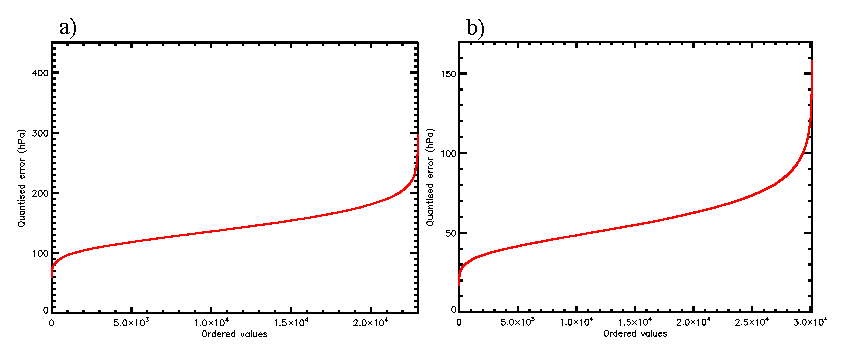
\includegraphics{Figures/SOM_orderedplot_lt20_regnl_cont}
\par\end{centering}

\caption{Ordered values for a) the whole domain and b) the continental domain
following filtering BMUs with a maximum grid discrepancy less than
20hPa. \label{fig:SOM-Ordered-histo-after-filt1}}
\end{figure}


Inspection of the BMU with the highest quantised error of the remaining
21,814 BMUs for the whole domain (Fig. \ref{fig:SOM-Comp-Aft-Filt2})
and of the remaining 28,602 for the continental domain (Fig. \ref{fig:SOM-Comp-Cont-Aft-Filt2})
revealed quite successful matches.
\begin{figure}[h]
\begin{centering}
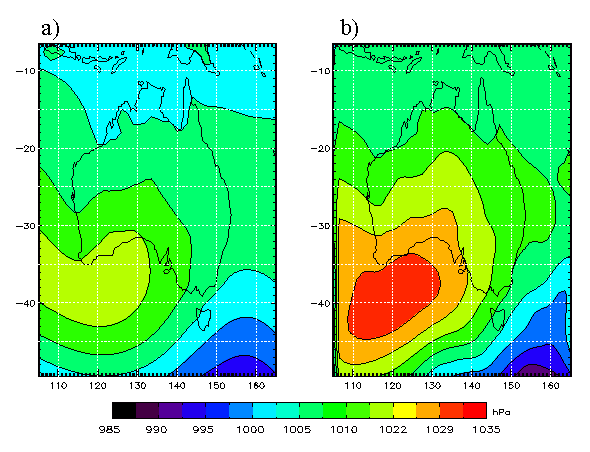
\includegraphics{Figures/SOM_comp_regnl_wrst_aft_filt_2}
\par\end{centering}

\caption{Comparison between a) node 28 from the SOM depicted in Fig. \ref{fig:6x5-SOM-space}
and b) the MSLP map from 1200UTC on July 18 2001. The quantised error
between a) and b) is 200.2hPa. The horizontal and vertical axes are
in units of degrees longitude and latitude, respectively. \label{fig:SOM-Comp-Aft-Filt2}}
\end{figure}
\begin{figure}[H]
\begin{centering}
\includegraphics{\string"/home/rhuva/Robert/Final Thesis/Chapter 5/Figures/SOM_cont_wrst_aft_filt_II\string".eps}
\par\end{centering}

\caption{Comparison between a) node three from the SOM depicted in Fig. \ref{fig:6x5-SOM-space-Cont}
and b) the MSLP map from 1800UTC on June 29 1995. The quantised error
between a) and b) is 90.9hPa. \label{fig:SOM-Comp-Cont-Aft-Filt2}}
\end{figure}


As the second filtering criterion relies upon the quantised error
measurement, which aggregates the error of the domain, it was then
decided that a final criterion be utilised to ensure that the remaining
BMUs were accurate enough with respect to the entire domain. The final
filtering criterion involved calculating the number of grid-points
from the BMU seen in Figs. \ref{fig:SOM-Comp-Aft-Filt2} and \ref{fig:SOM-Comp-Cont-Aft-Filt2}
that were more than 4hPa different from their respective MSLP map
from ERA-Interim (585 grid-points in the whole domain and 206 grid
points in the continental domain). The BMUs from the remaining 21,814/28,602
matches that had more than 585/206 grid points with an error greater
than 4hPa were then eliminated. This final criterion was used as a
method for checking the characteristics of the domain missed by the
quantised error measurement and left a total of 21,300 matches for
the whole domain and 28,572 matches for the continental domain. 

To determine the occurrence of the BMUs through time, the remaining
BMUs were compared with the original set of 30,680 and a BMU from
the original 30,680 that was eliminated through filtering was given
a missing value. The 21 years of BMUs was then reduced to a time series
of filtered BMUs and missing values. To give an indication of how
fragmented the time series of BMUs becomes after filtering, a histogram
of the number of consecutive time-steps without a BMU is presented
(Fig. \ref{fig:SOM-Consec-Zeros-Aft-Filt}a for the whole domain and
Fig \ref{fig:SOM-Consec-Zeros-Aft-Filt}b for the continental domain).
\begin{figure}[H]
\begin{centering}
\includegraphics{\string"/home/rhuva/Robert/Final Thesis/Chapter 5/Figures/SOM_cont_Consec_zeros_aft_filt\string".eps}
\par\end{centering}

\caption{Histogram of consecutive time-steps without a BMU after the final
filtering process for a) the whole domain and b) the continental domain.
\label{fig:SOM-Consec-Zeros-Aft-Filt}}
\end{figure}


Fig. \ref{fig:SOM-Consec-Zeros-Aft-Filt}a shows that although there
were some prolonged moments of missing data, which extend for more
than a few days at a time, the majority (78\%) of consecutive time-steps
without a matching BMU had a period less than a day for the whole
domain. The continental domain, with many more BMUs surviving filtering,
did much better in this respect with 98\% of periods with consecutive
missing time steps having a length of less than a day. The maximum
period without data was 12 days in length for the whole domain (1800UTC
on June 24 1990 up to and including 1200UTC July 6 1990) but as can
be seen from Fig. \ref{fig:SOM-Consec-Zeros-Aft-Filt} occurrences
of missing data that last more than two days are quite rare for both
SOMs. There was therefore no expectation that statistical testing
on monthly, seasonally or yearly time-scales would be adversely affected
by the missing data. 

However, given the ability for the SOM technique to, for the most
part, partition the MSLP data into easily classifiable synoptic regimes,
it does appear peculiar that there should exist a 12-day period in
which none of the SOM nodes from Fig. \ref{fig:6x5-SOM-space} were
able to describe the pressure distributions that occurred. The pressure
patterns during the 12 day period in winter of 1990 without SOM representation
therefore deserve further investigation. 


\subsubsection{Analysis of a 12-day SOM Failure\label{sub:Analysis-of-SOM-Fail}}

\begin{figure}[H]
\begin{centering}
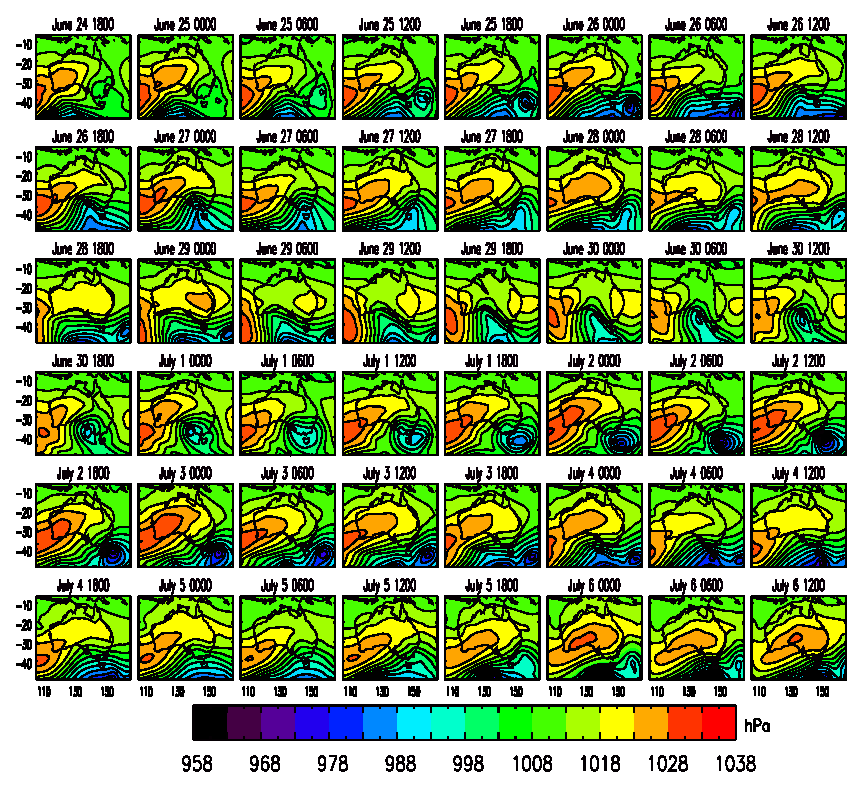
\includegraphics{Figures/12_day_gap_MSLP_data}
\par\end{centering}

\caption{Maps of ERA-Interim MSLP for the Australian region and for the period
1800UTC on June 24 1990 to 1200UTC on July 6 1990. \label{fig:MSLP-12day-SOM-Failure}}
\end{figure}


Fig. \ref{fig:MSLP-12day-SOM-Failure} depicts the pressure distributions
for the 12 day period of concern---1800UTC on June 24 1990 to 1200UTC
on July 6 1990 (hereafter referred to as 12B90). As can be seen from
Fig. \ref{fig:MSLP-12day-SOM-Failure} there were several cut-off
low pressure systems that affected southern parts of Australia, as
well as a rather deep and stationary high pressure centre south-west
of Perth for almost the entirety of 12B90. The position of the high
pressure centre in Fig. \ref{fig:MSLP-12day-SOM-Failure} is not considered
to be a common location for blocking to occur; blocking is more common
south-east of the continents in the southern hemisphere (\citealp{Sinclair1996};
\citealp{Mendes2008}). In fact, had the blocking high occurred in
one of the more common locations for blocking in the Australian region
SOM nodes six or 16 may have been suitable as BMUs. There are some
of the SOM nodes from Fig. \ref{fig:6x5-SOM-space} that have high
pressure centres resembling that of the blocking high in Fig. \ref{fig:MSLP-12day-SOM-Failure}.
However, none of the SOM nodes from Fig. \ref{fig:6x5-SOM-space}
have a high pressure centre that is deep enough or far enough south
to match the blocking high that occurred during 12B90. The associated
low pressure centres in Fig. \ref{fig:MSLP-12day-SOM-Failure} are
also quite intense on some of the days of 12B90 and these types of
cyclones are commonly filtered out due to the comparatively smooth
nature of the SOM nodes. 

The fact the high pressure centre was almost completely stationary
for 12 days during 12B90 also appears to be abnormal when compared
to previous research for the southern hemisphere (see \citealp{Sinclair1996};
\citealp{Mendes2008}; \citealp{Wiedenmann2002}). Analysis by \citet{Wiedenmann2002}
suggests that blocking normally lasts around five-seven days when
considering the domain of the Indian Ocean (roughly 30�-130�E and
south of 30�S), which indicates that blocking in almost the same position
for 12 days---like that in Fig. \ref{fig:MSLP-12day-SOM-Failure}---was
quite anomalous. To give an insight into the surface meteorological
conditions during 12B90, Fig. \ref{fig:12B90-Precip-Temp-Anom} shows
the temperature and precipitation anomalies at Perth (near the blocking
centre) and Melbourne (away from the blocking centre). 
\begin{figure}[H]
\begin{centering}
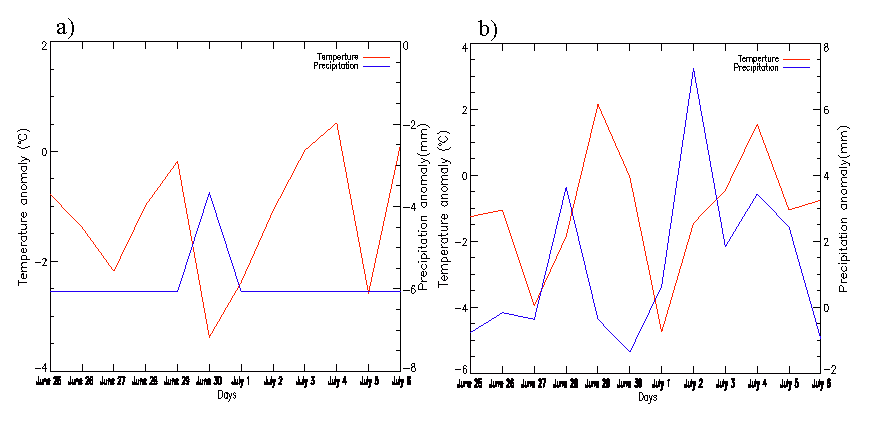
\includegraphics{Figures/gap_melb_maxtemp_precip_ts}
\par\end{centering}

\caption{Daily temperature and precipitation anomalies for the period June
25 to July 6 and for a) Perth and b) Melbourne. Anomalies are relative
to the average for that period using the BoM standard reference years
of 1961-1990. \label{fig:12B90-Precip-Temp-Anom}}
\end{figure}


As can be seen from Fig. \ref{fig:12B90-Precip-Temp-Anom}a Perth
was anomalously dry and cool during 12B90. Using the period of 1961-1990
the average daily rainfall for Perth during the days of 12B90 is about
6mm per day but only one day of rainfall totaling 2.4mm was recorded
during 12B90. The blocking of cold fronts and rain bearing systems
from reaching Perth, which is evident from Fig. \ref{fig:MSLP-12day-SOM-Failure},
is thus also evident in the rainfall anomalies for 12B90. In terms
of the conditions in Melbourne, Fig. \ref{fig:12B90-Precip-Temp-Anom}b
reveals a largely anomalously wet and cool-to-cold period during 12B90.
When considering the low pressure intrusions possible due to the position
of the blocking high in Fig. \ref{fig:MSLP-12day-SOM-Failure}, the
conditions in Melbourne are also not unexpected. These conditions
are also very similar to the pressure distributions identified in
\citet{Ashcroft2009} as cold-outbreak synoptic conditions. 


\section{Analysis of Regional and Continental SOMs\label{sub:Analysis-of-Regional}}

To give an indication as to the most commonly occurring SOM nodes
after filtering, Table. \ref{tab:SOM-Total-Occ} illustrates the total
occurrences of all nodes from the SOM depicted in Fig. \ref{fig:6x5-SOM-space}
(whole domain). 
\begin{table}[h]
\noindent \begin{centering}
\begin{tabular}{|c|c|c|c|c|c|c|}
\hline 
\multicolumn{7}{|c|}{Total occurrences (\%)}\tabularnewline
\hline 
\hline 
Row 0 & 3.67 & 3.96 & 4.28 & 4.21 & 3.31 & 3.36\tabularnewline
\hline 
Row 1 & 2.79 & 3.27 & 3.67 & 4.25 & 3.45 & 3.57\tabularnewline
\hline 
Row 2 & 1.74 & 2.51 & 3.48 & 3.46 & 3.40 & 3.76\tabularnewline
\hline 
Row 3 & 1.42 & 2.91 & 3.31 & 3.73 & 3.31 & 3.24\tabularnewline
\hline 
Row 4 & 2.03 & 3.22 & 3.57 & 4.04 & 4.16 & 2.91\tabularnewline
\hline 
 & Column 0 & Column 1 & Column 2 & Column 3 & Column 4 & Column 5\tabularnewline
\hline 
\end{tabular}
\par\end{centering}

\caption{Total occurrences of the SOM nodes from Fig. \ref{fig:6x5-SOM-space}
(whole domain). The numbers are as a percentage of the total number
of BMUs after filtering (21,300) and the row and column numbers correspond
to the rows and columns of Fig. \ref{fig:6x5-SOM-space}. \label{tab:SOM-Total-Occ}}
\end{table}
\begin{table}[h]
\noindent \centering{}%
\begin{tabular}{|c|c|c|c|c|c|c|}
\hline 
\multicolumn{7}{|c|}{Total occurrences (\%)}\tabularnewline
\hline 
\hline 
Row 0 & 3.29 & 2.84 & 3.42 & 3.51 & 2.80 & 2.18\tabularnewline
\hline 
Row 1 & 3.43 & 2.99 & 3.70 & 3.78 & 2.96 & 2.73\tabularnewline
\hline 
Row 2 & 3.86 & 3.06 & 3.59 & 4.18 & 3.52 & 3.31\tabularnewline
\hline 
Row 3 & 3.55 & 3.01 & 3.48 & 3.85 & 3.34 & 2.55\tabularnewline
\hline 
Row 4 & 3.27 & 3.13 & 3.67 & 4.56 & 3.76 & 2.71\tabularnewline
\hline 
 & Column 0 & Column 1 & Column 2 & Column 3 & Column 4 & Column 5\tabularnewline
\hline 
\end{tabular}\caption{As per Table. \ref{tab:SOM-Total-Occ} except for the continental
SOM, and where the total number of BMUs after filtering is 28,572.\label{tab:SOM-Cont-Total-Occ}}
\end{table}


Or in terms of a surface plot, the total occurrences of each node
can also be described by Fig. \ref{fig:SOM-Surf-Total-Occ} (whole
domain) and Fig. \ref{fig:SOM-Cont-Surf-Total-Occ} (continental domain).
\begin{figure}[H]
\begin{centering}
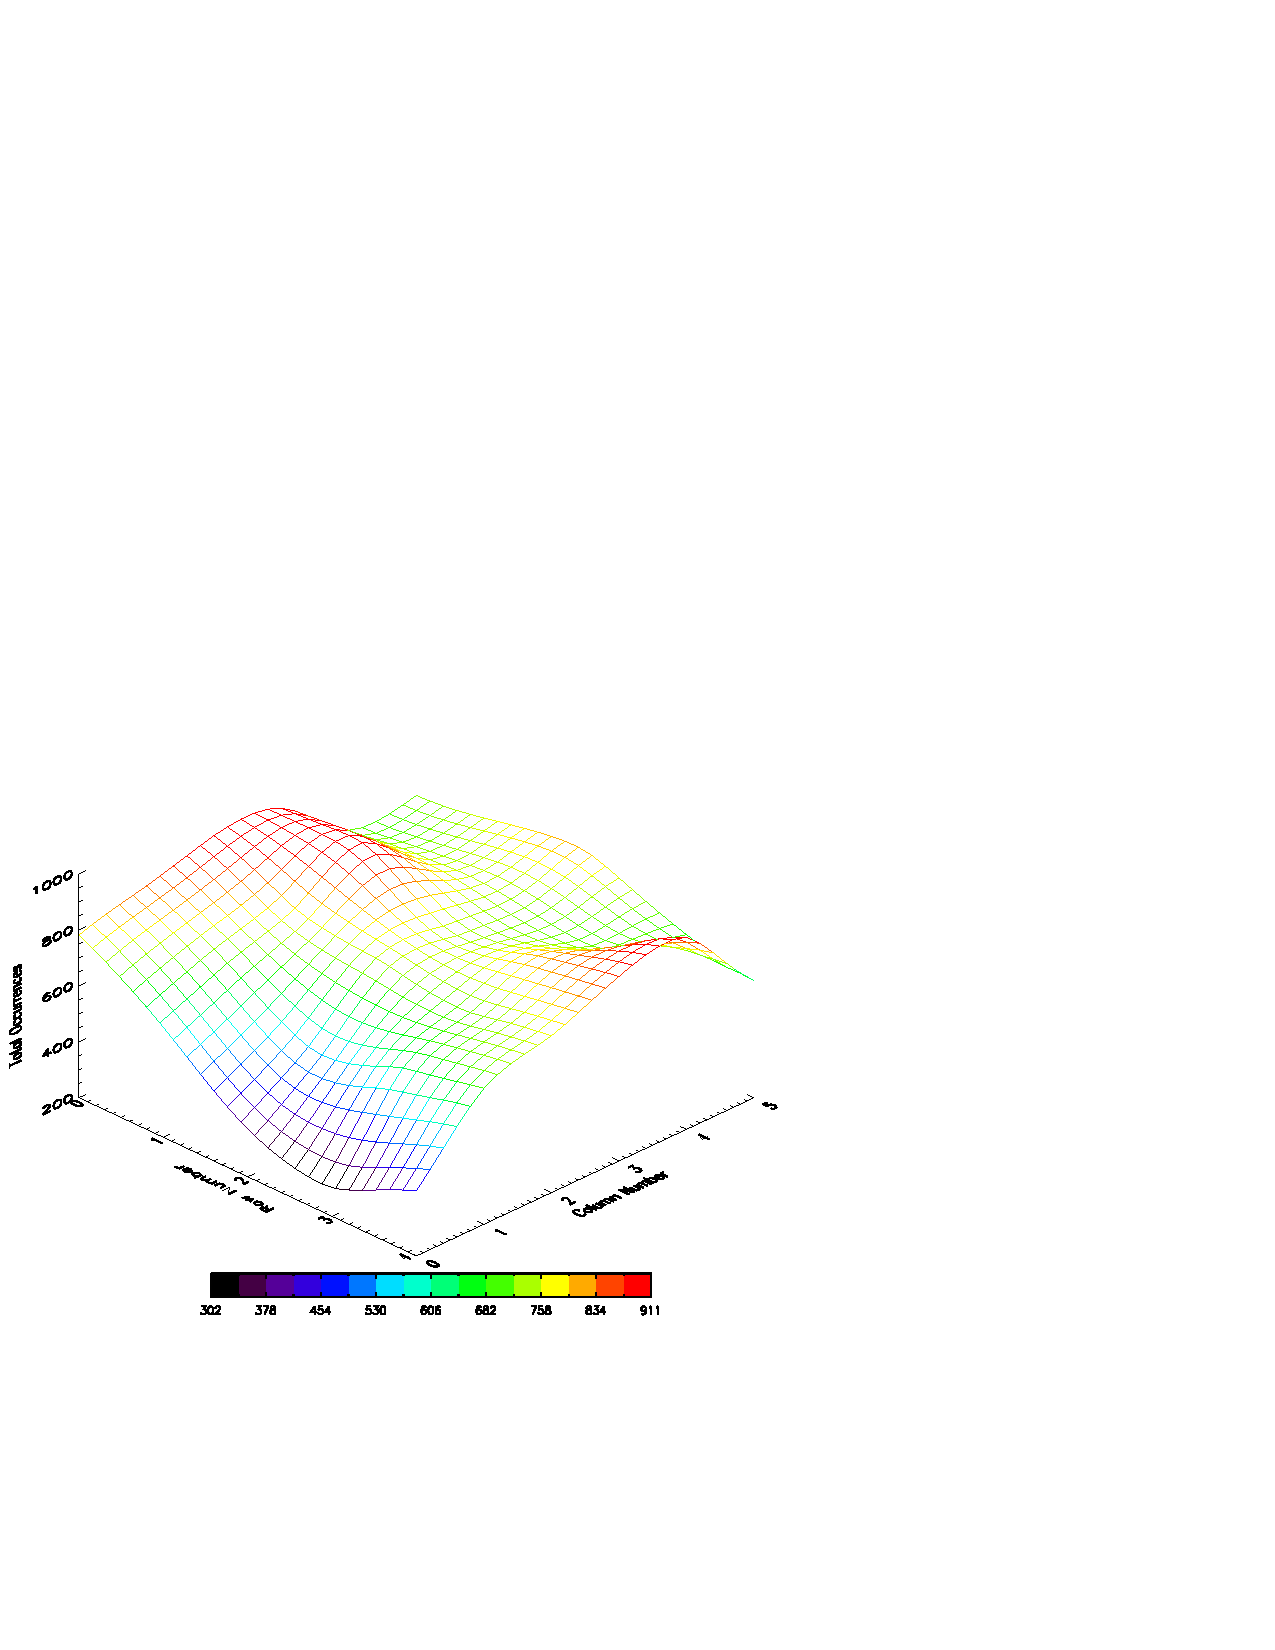
\includegraphics{Figures/SOM_regnl_total_occurrence_surface}
\par\end{centering}

\caption{Surface plot representing the total occurrences (after filtering)
of each SOM node from the SOM depicted in Fig. \ref{fig:6x5-SOM-space}
(whole domain). The row and column numbers correspond to the rows
and columns of Fig. \ref{fig:6x5-SOM-space}. \label{fig:SOM-Surf-Total-Occ}}
\end{figure}
\begin{figure}[H]
\begin{centering}
\includegraphics{\string"/home/rhuva/Robert/Final Thesis/Chapter 5/Figures/SOM_cont_surf_total_occ\string".eps}
\par\end{centering}

\caption{Surface plot representing the total occurrences (after filtering)
of each SOM node from the SOM depicted in Fig. \ref{fig:6x5-SOM-space-Cont}
(continental domain). The row and column numbers correspond to the
rows and columns of Fig. \ref{fig:6x5-SOM-space-Cont}. \label{fig:SOM-Cont-Surf-Total-Occ}}
\end{figure}


Fig. \ref{fig:SOM-Surf-Total-Occ} or Table. \ref{tab:SOM-Total-Occ}
show that the more commonly occurring whole domain SOM nodes were
those that involved high pressure systems located in either the Bight
or south of Perth. Similarly, the most commonly occurring continental
SOM nodes were nodes 28 and 16, which both involve higher pressures
to the south. Least common were the SOM nodes that involved low pressure
intrusions south of Victoria or South Australia (both whole and continental
domains), although this statistic was easily explained given the fast-moving
nature of low pressure systems in comparison to high pressure systems
(\citealp{Sturman2005}). A more important result was the fact that
the SOM technique, in this case, was able to identify the seasonality
of the Australian region. 
\begin{figure}[H]
\begin{centering}
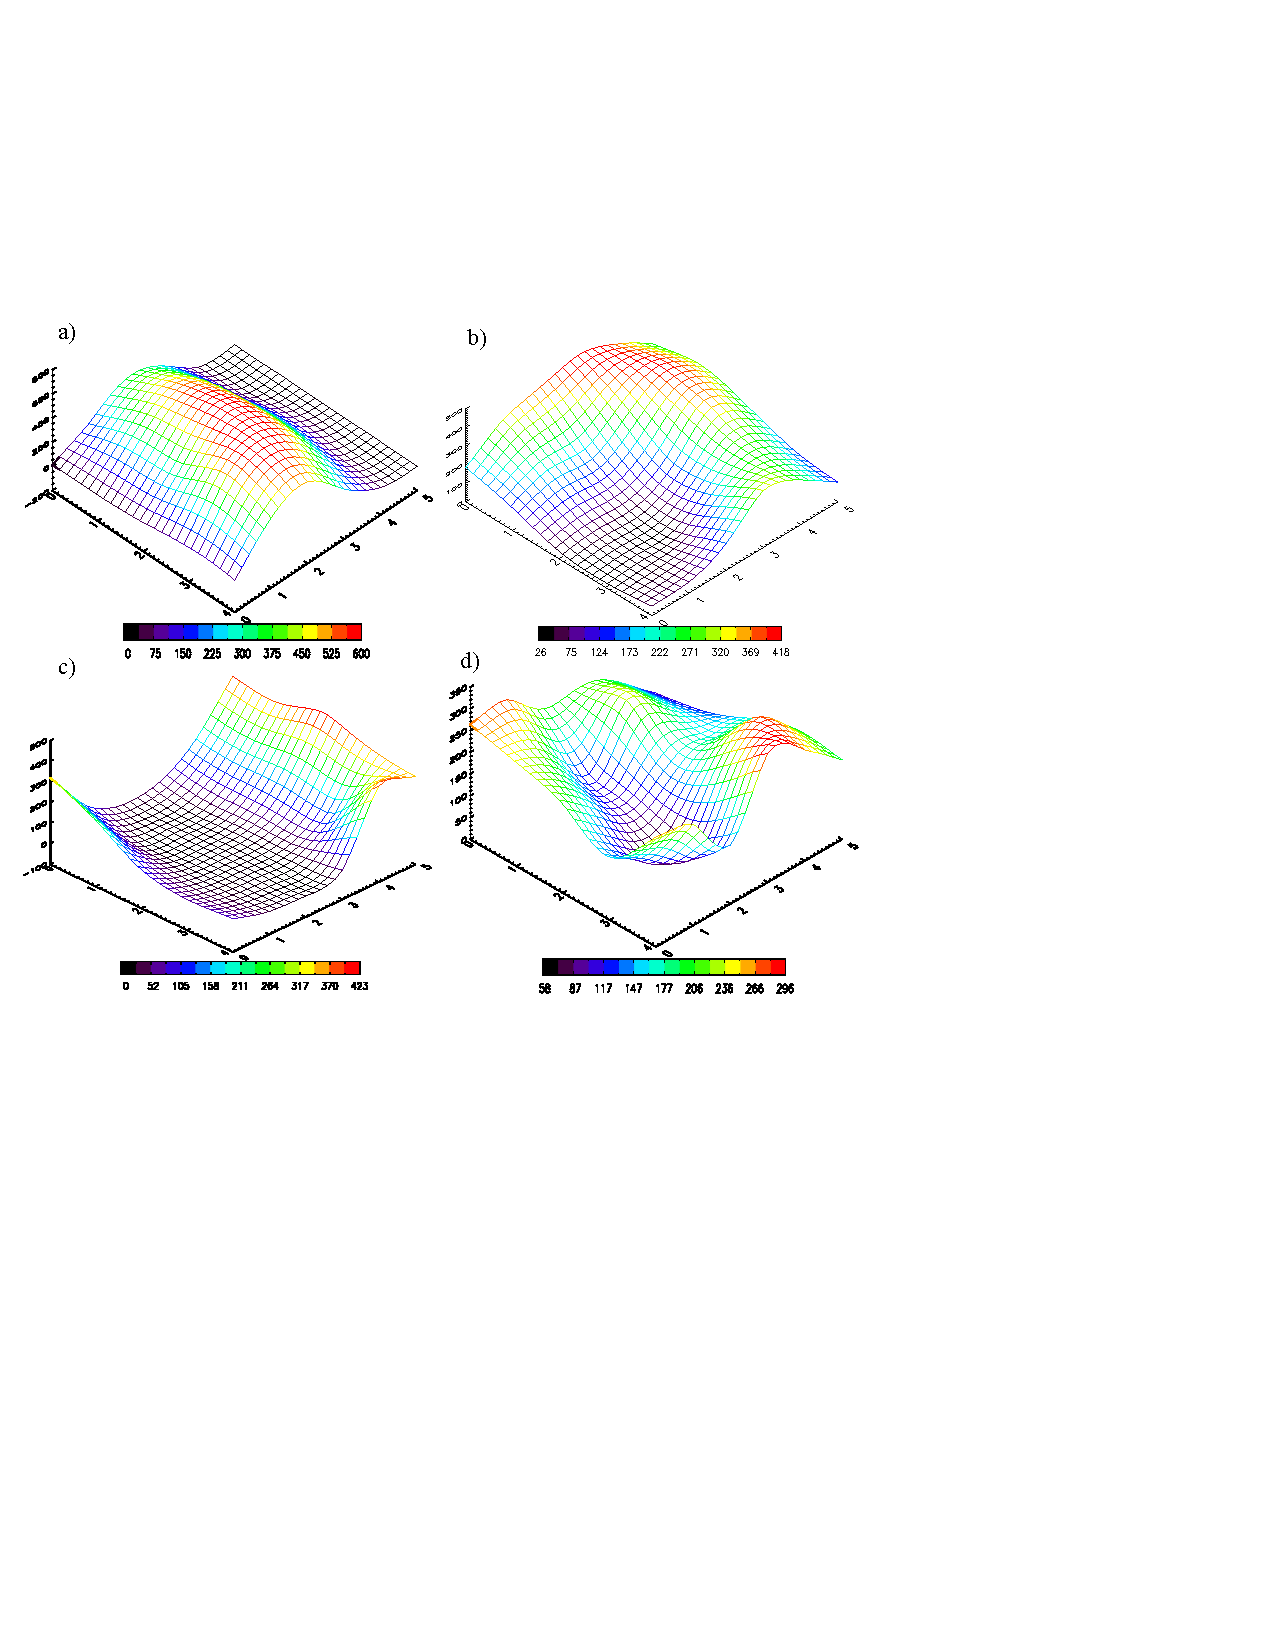
\includegraphics{Figures/SOM_regnl_all-seasons_occurrence_surface}
\par\end{centering}

\caption{Seasonal occurrences of the SOM nodes depicted in Fig. \ref{fig:6x5-SOM-space}
(whole domain). Totals are after filtering while a) is summer, b)
is autumn, c) is winter and d) is spring. The row and column numbers
correspond to the rows and columns of Fig. \ref{fig:6x5-SOM-space}.
\label{fig:SOM-Surf-Seasnl-Occ}}
\end{figure}
\begin{figure}[h]
\begin{centering}
\includegraphics{\string"/home/rhuva/Robert/Final Thesis/Chapter 5/Figures/SOM_cont_surf_all_seasons_occ\string".eps}
\par\end{centering}

\caption{Seasonal occurrences of the SOM nodes depicted in Fig. \ref{fig:6x5-SOM-space-Cont}
(continental domain). Totals are after filtering while a) is summer,
b) is autumn, c) is winter and d) is spring. The row and column numbers
correspond to the rows and columns of Fig. \ref{fig:6x5-SOM-space-Cont}.
\label{fig:SOM-Cont-Surf-Seasnl-Occ}}
\end{figure}


As can be seen from both Figs. \ref{fig:SOM-Surf-Seasnl-Occ} and
\ref{fig:SOM-Cont-Surf-Seasnl-Occ} the SOM nodes that occur in summer
do not occur in winter, but the difference between spring and autumn
is less defined. The summer nodes generally involve high pressure
systems and transitions between successive highs to the south of the
continent (centred \textasciitilde{} 40�S). Conversely, the winter
nodes are those that involve deeper high pressure systems than in
summer and high pressure systems that are centred more over the Australian
continent (\textasciitilde{}30-35�S). Importantly, the implied summer-only
and winter-only nodes from Fig. \ref{fig:SOM-Surf-Seasnl-Occ} correspond
well with previous findings from \citet{Alexander2010} and \citet{Meteorology2011a}
as characteristic MSLP distributions for the Australian region during
summer and winter. 

One of the key differences between the SOM technique and other statistical
techniques (e.g. clustering) involves the SOM\textquoteright{}s ability
to span the data-space. Because each SOM node is closely related to
its surrounding nodes there is an expectation that transition maps
should reveal the temporal evolution of synoptic events across the
region. For instance, one might expect that the west-east progression
of synoptic weather systems in the mid-latitudes be easily determined
from such a plot of SOM node transitions. However, in the current
study such clearly defined transitions were not possible (Fig. \ref{fig:SOM-Transition-and-Stationary}a)
and it was thought this could have been because the SOM used was too
large and therefore containing too many intermediate synoptic states.
\begin{figure}[H]
\begin{centering}
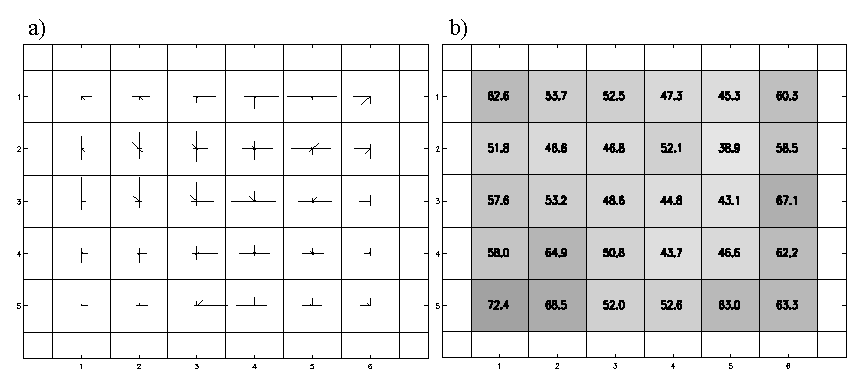
\includegraphics{Figures/SOM_regnl_Forward-and-No_transitions}
\par\end{centering}

\caption{Plots showing a) the forward transitions between SOM nodes after filtering,
and b) percentages of occurrences where no transition is made. Vectors
in a) are normalised according to the total occurrences of each node
and the row and column numbers correspond to the rows and columns
of the SOM in Fig. \ref{fig:6x5-SOM-space} (whole domain). Darker
grey in b) indicates larger values. \label{fig:SOM-Transition-and-Stationary}}
\end{figure}


But more likely, the temporal resolution of the data used was responsible
for the lack of clear transitions in Fig. \ref{fig:SOM-Transition-and-Stationary}a.
The use of six-hourly MSLP data in the current study has most likely
led to less linear paths being traced out across the SOM space, thus
leading to a less consistently unidirectional transition plot (which
is evident in the high percentage of no transitions seen in Fig. \ref{fig:SOM-Transition-and-Stationary}b).
Analysis of MSLP data at 12-hourly or daily intervals, like that in
\citet{Hewitson2002}, could have led to transition plots with a more
clearly defined cycle of high-low pressure systems. 


\section{Conclusion\label{sec:SOM-Conclusion}}

Despite the limitations of the SOM technique, which are similar to
the problems encountered with most data synthesis techniques, a SOM
of the MSLP in the Australian region was able to identify commonly
occurring and previously identified MSLP pressure patterns, or synoptic
regimes (whole domain). Using the MSLP field, even though it may not
have an immediately obvious connection to the wind and solar fields,
for categorising the weather into regimes was an important process
towards identifying commonly co-occurring wind and solar conditions.
Converting the continuous time series of ERA-Interim weather conditions
into a time series of 30 SOM nodes will allow for an analysis of the
wind and solar conditions under each SOM node. Removal of the ocean
MSLP data was also undertaken and an alternative continental SOM presented.
The continental analysis, despite the limited domain, was able to
produce a set of SOM nodes that contained features consistent with
the Australian region, while at the same time achieved a much more
continuous representation of the ERA-Interim data (93\% of time-steps
had a BMU). Importantly, the removal of ocean grid-points rids the
domain of a large source of error (for instance, the transient low
pressure centre seen in Fig. \ref{fig:SOM-comp-worst-before}b). With
a vastly more complete representation of the data from ERA-interim
by the continental SOM a more comprehensive analysis of the concurrent
wind and solar conditions associated with each SOM node is possible. 
\end{document}
